% Compile with XeLaTeX or LuaLaTeX
\documentclass[14pt,a4paper]{extreport}

% -------------------------
% Language and font setup
% -------------------------
\usepackage{fontspec}
\usepackage{polyglossia}
\setmainlanguage{russian}
\setotherlanguage{english}

\defaultfontfeatures{Ligatures=TeX}
\setmainfont{Times New Roman}
\setsansfont{Arial}
\setmonofont{Courier New}
\newfontfamily\cyrillicfont{Times New Roman}
\newfontfamily\cyrillicfontsf{Arial}
\newfontfamily\cyrillicfonttt{Courier New}

% -------------------------
% Page layout
% -------------------------
\usepackage[
    a4paper,
    left=25mm,   % left margin >= 20mm
    right=15mm,
    top=20mm,
    bottom=20mm
]{geometry}

% -------------------------
% Paragraph formatting
% -------------------------
\usepackage{setspace}
\setstretch{1.5}                 % allowed range: 1.3--1.5
\setlength{\parindent}{1cm}      % red line / paragraph indentation
\setlength{\parskip}{0pt}

\usepackage{ragged2e}
\justifying

\emergencystretch=3em

% -------------------------
% Math, figures, tables
% -------------------------
\usepackage{amsmath, amssymb}
\usepackage{graphicx}
\usepackage{float}
\usepackage{booktabs}
\usepackage{array}
\usepackage{longtable}
\usepackage{caption}
% \usepackage{chngcntr}

% Number figures, tables, and equations inside chapters: 2.3, 2.4, etc.
\numberwithin{figure}{chapter}
\numberwithin{table}{chapter}
\numberwithin{equation}{chapter}

% Figure captions: below, centered, "Рис. 2.3."
\captionsetup[figure]{
    name=Рис.,
    labelsep=period,
    justification=centering,
    singlelinecheck=false
}

% Table captions: above, right-aligned, "Таблица 2.3."
\captionsetup[table]{
    name=Таблица,
    labelsep=period,
    justification=raggedleft,
    singlelinecheck=false,
    position=top
}

% -------------------------
% Section heading formatting
% -------------------------
\usepackage{titlesec}

\titleformat{\chapter}
    {\normalfont\bfseries\centering}
    {\thechapter}
    {1em}
    {}

\titleformat{\section}
    {\normalfont\bfseries}
    {\thesection}
    {1em}
    {}

\titleformat{\subsection}
    {\normalfont\bfseries}
    {\thesubsection}
    {1em}
    {}

\usepackage{minted}
\usepackage{xcolor}

\definecolor{codebg}{HTML}{EEEEE8}

\setminted{
  bgcolor=codebg,
  fontsize=\small,
  breaklines=true,
  frame=none,
  framesep=2mm,
  xleftmargin=2em,
  style=tango
}

\usepackage[ruled,vlined,linesnumbered,algochapter]{algorithm2e}
\SetAlgorithmName{Алгоритм}{алгоритм}{Список алгоритмов}

% -------------------------
% Table of contents formatting
% -------------------------
\usepackage{tocloft}
\renewcommand{\contentsname}{Содержание}

% -------------------------
% Bibliography: GOST-style references
% -------------------------
\usepackage[
    backend=biber,
    style=gost-numeric,
    sorting=none
]{biblatex}

\addbibresource{references.bib}

% -------------------------
% Hyperlinks and cross-references
% -------------------------
\usepackage[hidelinks]{hyperref}

% -------------------------
% Appendix formatting
% -------------------------
\usepackage{appendix}

\renewcommand{\appendixname}{Приложение}
\renewcommand{\appendixtocname}{Приложения}
\renewcommand{\appendixpagename}{Приложения}

% -------------------------
% Helper commands
% -------------------------

% Unnumbered annotation page
\newcommand{\annotationpage}[2]{
    \clearpage
    \thispagestyle{empty}
    \begin{center}
        \textbf{#1}
    \end{center}

    #2
}

% Standard chapter conclusion section
\newcommand{\chapterconclusions}{
    \section{Выводы по главе}
}

% Formula legend helper
\newenvironment{formulalegend}{
    \par\noindent\textit{где:}
    \begin{itemize}
}{
    \end{itemize}
}

% -------------------------
% Document begins
% -------------------------
\begin{document}

% =========================================================
% Title page: not numbered
% =========================================================
\pagenumbering{gobble}

\begin{titlepage}
    \thispagestyle{empty}
    \setstretch{1.0}
    \small

    \begin{center}
        \textbf{ФЕДЕРАЛЬНОЕ ГОСУДАРСТВЕННОЕ АВТОНОМНОЕ ОБРАЗОВАТЕЛЬНОЕ УЧРЕЖДЕНИЕ}\\
        \textbf{ВЫСШЕГО ОБРАЗОВАНИЯ}\\
        \textbf{«НАЦИОНАЛЬНЫЙ ИССЛЕДОВАТЕЛЬСКИЙ УНИВЕРСИТЕТ}\\
        \textbf{«ВЫСШАЯ ШКОЛА ЭКОНОМИКИ»}\\[0.3cm]

        \textbf{ФАКУЛЬТЕТ КОМПЬЮТЕРНЫХ НАУК}\\[1.4cm]

        Нигматуллин Роман Максимович \\[1.0cm]

        \textbf{МАГИСТЕРСКАЯ ДИССЕРТАЦИЯ}\\[0.6cm]

        \textbf{Методы поиска кандидатов на графических ускорителях в рекомендательных системах}\\[0.25cm]
        \textbf{GPU Retrieval in Recommender Systems}\\[1.0cm]

        по направлению подготовки \underline{01.04.02 Прикладная математика и информатика}\\
        образовательная программа \underline{«Современные Компьютерные Науки»}
    \end{center}

    \vspace{0.9cm}

    \begin{flushright}
        \begin{tabular}{l}
            Научный руководитель\\
            Младший научный сотрудник\\
            [0.35cm]
            \rule{7cm}{0.4pt}\\
            К.Я. Хрыльченко \\[1cm]

            Студент\\
            [0.35cm]
            \rule{7cm}{0.4pt}\\
            Р.М. Нигматуллин
        \end{tabular}
    \end{flushright}

    \vfill

    \begin{center}
        Москва \the\year
    \end{center}
\end{titlepage}

% =========================================================
% Russian annotation
% =========================================================
\annotationpage{Аннотация}{
Поиск кандидатов в современных рекомендательных системах требует высокой скорости, поддержки строгой атрибутной фильтрации и экономии памяти. Существующие ANN-библиотеки для GPU не интегрируются в PyTorch-граф, вызывают разрывы вычислительного графа с переключением на CPU и зачастую не имеют гибкой встроенной фильтрации.

В работе представлен \textbf{torchretrieve} --- открытый фреймворк на базе PyTorch и Triton для эффективного поиска на GPU с поддержкой \textbf{torch.compile}. В нём реализованы алгоритмы LiNR (V1--V3), их новая INT8-версия (V4), а также новый алгоритм QuantizedIVF, объединяющий кластеризацию, INT8-квантизацию и фильтрацию в виде ядра Triton.

Эксперименты на наборах данных Goodreads, arXiv и Yambda (до 5 млрд взаимодействий) показали, что со встроенной фильтрацией QuantizedIVF ускоряет поиск на порядок при сохранении 76--94\% полноты (Recall). Алгоритм LiNR V4 двукратно снижает потребление памяти при $\ge$95\% полноты. В режиме без фильтрации методы почти не уступают точному поиску, а при наличии атрибутных ограничений предложенные методы со встроенной фильтрацией успешно решают проблему нехватки кандидатов (liquidity problem), свойственную классическим ANN с постфильтрацией, выступая эффективной альтернативой полному перебору. Исходный код и результаты опубликованы открыто, решая проблему воспроизводимости.
}

% =========================================================
% English annotation
% =========================================================
\annotationpage{\textenglish{Abstract}}{
\begin{english}
Candidate retrieval in modern recommender systems requires high speed, strict attribute filtering, and memory efficiency. Existing GPU-based ANN libraries do not integrate into the PyTorch graph, cause computational graph breaks with CPU synchronization, and often lack flexible inline filtering.

This thesis presents \textbf{torchretrieve}, an open-source PyTorch and Triton framework for efficient GPU retrieval supporting \textbf{torch.compile}. It implements the LiNR algorithms (V1--V3), a novel INT8-quantized variant (V4), and a new QuantizedIVF algorithm combining clustering, INT8 quantization, and Bloom filtering into a single kernel.

Evaluations on Goodreads, arXiv, and Yambda datasets (up to 5 billion interactions) show that under inline filtering, QuantizedIVF achieves an order-of-magnitude speedup while maintaining 76--94\% recall. The LiNR V4 variant halves memory consumption while preserving $\ge$95\% recall. In the unfiltered regime, the methods perform on par with exact search, while under attribute constraints, the proposed methods with inline filtering successfully solve the liquidity problem inherent to classical post-filtering ANN, serving as an effective alternative to exhaustive search. The source code and experimental results are publicly released, solving the reproducibility problem.
\end{english}
}

% =========================================================
% Main part starts here
% =========================================================
\clearpage
\pagenumbering{arabic}

\tableofcontents
\clearpage

% =========================================================
% Introduction
% =========================================================
\chapter*{Введение}
\addcontentsline{toc}{chapter}{Введение}

Современные рекомендательные системы часто используют двухстадийную архитектуру, в которой первый этап поиска кандидатов сужает каталог из $10^6$--$10^9$ объектов до набора кандидатов размером $10^2$--$10^3$, после чего этот набор обрабатывается более сложными моделями ранжирования \cite{covington2016deep, yi2019sampling}. Этап поиска кандидатов, или генерация кандидатов, имеет жёсткие требования по скорости --- от нескольких миллисекунд до сотни миллисекунд на запрос в масштабных рекомендательных системах --- и определяет потолок полноты (Recall) всего конвейера: объекты, которые он не извлёк, не могут быть восстановлены последующим переранжированием. Одним из самых вычислительно дорогих этапов этой стадии является векторный поиск --- алгоритм нахождения $K$ объектов с наибольшим скалярным произведением (или другой функцией расстояния) между эмбеддингом запроса и эмбеддингом объекта; для этой операции известно большое число методов приближённого поиска ближайших соседей (ANN) \cite{jegou2011product, ootomo2024cagra, wang2021milvus, zhao2020song}.

До недавнего времени экосистема ANN-алгоритмов и векторных баз данных строилась на предположении о том, что поиск кандидатов --- это \textit{статический поиск по индексу}: индекс строится предварительно в отдельном процессе, запрос не имеет дополнительных условий для фильтрации, а единственным результатом является набор из $K$ лучших по сходству объектов. Современные высоконагруженные рекомендательные и поисковые системы ради более высокого качества и скорости ответа обязаны обладать свойствами, при которых эти предположения нарушаются. Во-первых, поиск кандидатов выполняется с учетом фильтрации по различным атрибутам: музыкальная рекомендательная система должна учитывать ограничения по языку, региону и лицензии; книжная --- фильтровать по жанру, году и языку; поиск по научной литературе --- ограничивать по тематике, времени публикации, категории. Обычные алгоритмы ANN с постфильтрацией страдают резким падением полноты при высокой селективности фильтра, поскольку отфильтрованные объекты занимают позиции в списке кандидатов; эту проблему нехватки релевантных кандидатов (в оригинале --- «liquidity problem») выделили в работе \cite{borisyuk2024linr}. Во-вторых, как таблица эмбеддингов, так и веса модели всё чаще развертываются в одном сервисе, а не изолированно: в статье LiNR компании LinkedIn поиск кандидатов выражается как один вызов модуля \textbf{nn.Module}, который содержит и таблицу эмбеддингов, и индексы атрибутов для фильтрации, а также проводит вычисления скалярных произведений прямо в коде модели-энкодера, предоставляющей эмбеддинг запроса \cite{borisyuk2024linr}. В-третьих, размер каталогов в современных рекомендательных системах достигает миллиардов объектов, а размерность эмбеддингов постоянно увеличивается. В таких сценариях основным ограничивающим фактором оказываются уже не только тяжелые вычисления, но и пропускная способность различных видов памяти процессоров и ускорителей; это мотивирует переход к низкобитным схемам квантизации или приближенным алгоритмам, сохраняющим качество при сжатии индекса в несколько раз \cite{li2023oporp, nvidia2024cuda}.

Библиотеки на языке CUDA, доминирующие сегодня в области ANN на GPU, и применяющие их системы --- NVIDIA CAGRA \cite{ootomo2024cagra}, Milvus \cite{wang2021milvus}, SONG \cite{zhao2020song} --- не предоставляют интеграции с моделью PyTorch и не встраиваются в её граф, из-за чего для их использования в рекомендательной системе необходима десериализация, синхронизация различных стадий и даже пересылка данных по сети в процессе построения списка объектов. Из-за этого различные компоненты нейросетевых моделей необходимо разбивать на подграфы, балансировать ресурсы CPU и GPU, контролировать доступность сразу нескольких сервисов. Кроме того, они накладывают жёсткие ограничения на количество кандидатов и не предоставляют встроенного средства для фильтрации по атрибутам, к которому ядро поиска могло бы обращаться напрямую, либо имеют такой функционал только для CPU. Известные индустриальные системы, решающие эту задачу --- в первую очередь LiNR \cite{borisyuk2024linr} --- хоть и описаны в научных статьях, но являются проприетарными. В экосистеме PyTorch нет открытой библиотеки, в которой были бы воспроизведены промышленные алгоритмы или предложены альтернативы под унифицированным интерфейсом; закрытое программное обеспечение, описанное в статьях, тяжело воспроизвести и оценить его качество на открытых наборах данных, что создает барьер для воспроизводимости.

В работе рассматривается только этап поиска кандидатов, в частности --- векторный поиск по эмбеддингам объектов как один из самых распространённых способов реализации этого этапа. Цель работы --- создать фреймворк с реализациями алгоритмов поиска кандидатов с поддержкой фильтрации, которые работают на различном аппаратном обеспечении (включая разные видеокарты), не требуют длительной компиляции CUDA-кода и за счёт использования языка Triton легко встраиваются в существующие проекты на PyTorch. В библиотеке представлены алгоритмы LiNR V1--V3 \cite{borisyuk2024linr}, дополненные квантизованным INT8-вариантом, названным V4, а также алгоритм QuantizedIVF --- предложенная в данной работе реализация популярного алгоритма приближенного поиска в PyTorch с поддержкой графических ускорителей.

Для достижения поставленной цели в рамках работы была подготовлена реализация алгоритмов LiNR и QuantizedIVF на базе фреймворка PyTorch. Для повышения эффективности работы с памятью ряд модулей был переписан с использованием вычислительных ядер на языке Triton. Оценка качества и скорости алгоритмов проводится с помощью специально разработанного конфигурируемого Python-модуля. В качестве энкодеров применяются gSASRec \cite{petrov2023gsasrec} для рекомендательных наборов данных и предобученная текстовая модель Nomic-Embed \cite{nussbaum2024nomic} для семантического поиска на наборе arXiv. Экспериментальная часть охватывает три набора данных, три различные размерности эмбеддингов и пять алгоритмов в одной или двух реализациях. По результатам тестирования построены Парето-кривые, отражающие соотношение качества, скорости и потребления памяти в различных условиях. Исходный код фреймворка, конфигурации экспериментов, эталоны точного поиска и полученные результаты выложены в открытый репозиторий на GitHub \cite{torchretrieve_repo}.

Оценка алгоритмов проводилась с учетом специфики режимов поиска кандидатов. Для тестирования встроенной фильтрации использовались наборы данных (датасеты) Goodreads \cite{wan2018item, wan2019fine} и arXiv \cite{clement2019arxiv}, содержащие атрибуты различной гранулярности. Режим без фильтрации оценивался на наборе Yambda \cite{yandex2025yambda} в масштабах 500 миллионов и 5 миллиардов событий, что позволило проанализировать масштабируемость алгоритмов и изменение скорости ответа при существенном увеличении размера каталога.

Результаты экспериментов показали, что в режиме со встроенной фильтрацией алгоритм QuantizedIVF способен ускорить работу на порядок при сохранении 76--94\% полноты относительно точного поиска KNN с фильтром. В свою очередь, квантизованный INT8-вариант V4 позволяет вдвое уменьшить объем памяти индекса, обеспечивая полноту не ниже 95\%. При тестировании в режиме без фильтрации приближённые алгоритмы продемонстрировали практически полное отсутствие потерь в качестве по сравнению с базовым методом.

Дальнейшая структура работы выстроена следующим образом. Во второй главе приводится обзор литературы по промышленному поиску кандидатов, классическим методам ANN и их адаптации для GPU, а также вопросам атрибутной фильтрации и квантизации эмбеддингов. В третьей главе дается формальное описание рассматриваемых алгоритмов. Четвертая глава раскрывает архитектурные решения разработанного фреймворка. В пятой главе подробно описываются используемые наборы данных, энкодеры и методология оценки. Шестая глава содержит результаты проведенных экспериментов, а в заключительной седьмой главе подводятся итоги работы и обозначаются направления для дальнейших исследований.

% =========================================================
% Chapter 2
% =========================================================
\chapter{Обзор предметной области}

\section{Поиск кандидатов в современных рекомендательных системах}

Двухэтапная архитектура стала индустриальным стандартом для построения масштабных рекомендательных систем. Первое широко известное описание этого подхода было представлено в работе Ковингтона и соавторов \cite{covington2016deep} на примере рекомендательной системы YouTube, где на первом этапе из миллионного корпуса отбирается несколько сотен релевантных видео, которые затем оцениваются более сложной моделью ранжирования. Доминирующей архитектурой этапа генерации кандидатов выступает двухбашенная (two-tower) модель. В ней профиль пользователя и характеристики объекта независимо проецируются в общее векторное пространство, благодаря чему задача поиска сводится к нахождению пар с наибольшим скалярным произведением. Исторически этот подход восходит к архитектуре Deep Structured Semantic Model (DSSM) \cite{huang2013learning}, изначально предложенной для задач веб-поиска. Впоследствии он был существенно улучшен: например, в работе \cite{yi2019sampling} предложен метод коррекции смещения выборки, что сделало возможным эффективное обучение двухбашенных моделей на сверхбольших корпусах данных.

Несмотря на свою популярность, стандартный векторный поиск обладает рядом ограничений: он опирается лишь на простую оценку геометрического сходства, не поддерживает встроенную атрибутную фильтрацию и не позволяет проводить совместную оптимизацию с этапом ранжирования. Эти недостатки стимулируют развитие методов поиска кандидатов непосредственно на GPU с использованием логики самой модели, что будет подробно рассмотрено в разделе 2.4. В рамках данной работы фокус внимания и все эксперименты сосредоточены исключительно на повышении качества и производительности первого этапа, тогда как этап итогового ранжирования остается за рамками исследования.

\section{Последовательные энкодеры для эмбеддингов запросов}

В современных рекомендательных системах за формирование эмбеддинга запроса обычно отвечает энкодер над историей пользовательских взаимодействий с объектами (просмотры, нажатия, покупки, добавления в избранное). Эта модель принимает на вход историю взаимодействий пользователя и агрегирует её в единый вектор, необходимый для предсказания следующего релевантного объекта. Развитие архитектур на базе трансформеров в этой области во многом началось с модели SASRec \cite{kang2018self}, успешно адаптировавшей механизм внутреннего внимания (self-attention) для задачи предсказания следующего элемента последовательности. До сих пор SASRec остается одним из самых сильных и надежных базовых решений. Дальнейшим развитием этой идеи стала архитектура BERT4Rec \cite{sun2019bert4rec}, в которой постановка задачи была расширена до двунаправленного обучения с маскированием токенов по аналогии с языковыми моделями.

В качестве основного энкодера в данной работе используется модель gSASRec \cite{petrov2023gsasrec}. В оригинальной статье авторы выявили проблему нестабильности при обучении классического SASRec с использованием бинарной кросс-энтропии и сэмплирования отрицательных примеров: модель склонна сходиться к экстремально большим значениям логитов. Для решения этой проблемы в gSASRec предложена модифицированная функция потерь, которая репараметризует правдоподобие таким образом, что эффективная частота сэмплирования явно учитывается в целевой функции. В контексте нашего исследования моделирование самих наборов данных и эксперименты с методологией обучения не являются целью, а выбор gSASRec обусловлен тем, что эта архитектура обеспечивает быструю и стабильную сходимость при обучении. Использование надежного энкодера позволяет исключить влияние нестабильности модели на итоговые метрики и сосредоточиться исключительно на сравнении алгоритмических особенностей и производительности методов поиска в главе 6.

\section{Классический ANN и ANN на GPU}

Исторически алгоритмы приближенного поиска ближайших соседей (ANN) развивались в двух основных направлениях: методы на основе квантизации и методы на основе графов. Одним из базовых и наиболее востребованных на практике подходов в первом направлении является скалярная квантизация (Scalar Quantization, SQ). Идея SQ заключается в независимом сжатии каждой компоненты вектора высокой размерности --- как правило, путем перевода значений с плавающей точкой в низкобитный целочисленный формат (например, INT8). В сочетании с инвертированным файлом (структура IVF) этот подход позволяет существенно сократить объем потребляемой памяти и ускорить вычисление расстояний за счет использования быстрой целочисленной арифметики. Существуют и более специфичные методы квантизации, разработанные для конкретных задач --- так, в алгоритме ScaNN \cite{guo2020accelerating} была предложена анизотропная квантизация, при которой вместо обычной минимизации ошибки восстановления вектора, сжатие оптимизируется так, чтобы сохранить правильный порядок скалярных произведений.

Доминирующей альтернативой методам квантизации стали алгоритмы на основе графов, среди которых стандартом является HNSW (Hierarchical Navigable Small World) \cite{malkov2020efficient}. В HNSW все векторы раскладываются в иерархическую систему слоев так, чтобы каждый слой был small-world графом и между любыми двумя векторами в слое существовал короткий путь, а при поиске обходим этот граф жадным алгоритмом. Графовые подходы имеют высокую полноту и скорость на CPU, а также масштабируются до миллиардов векторов за счет выгрузки во внешнюю память \cite{subramanya2019diskann}.

С развитием нейросетей большинство рекомендательных систем стали активно использовать графические ускорители (GPU) --- специальные процессоры с поддержкой параллелизма и высокой пропускной способностью памяти, которые идеально подходят для матричных вычислений (как 
в IVF), но плохо справляются с ветвлениями в алгоритмах и случайным доступом к памяти, характерными для HNSW.
Тем не менее, в стеке NVIDIA был разработан алгоритм CAGRA \cite{ootomo2024cagra} --- наиболее значимый на 
сегодняшний день графовый ANN на GPU. CAGRA перерабатывает структуру графа таким образом, чтобы минимизировать 
расхождение потоков (warp divergence) и оптимизировать паттерны доступа к памяти, обеспечивая построение индекса и поиск 
целиком на видеокарте.

Помимо графовых подходов, активно развиваются векторные базы данных и системы, адаптирующие кластеризацию под GPU. 
Например, Milvus \cite{wang2021milvus} предоставляет комплексную инфраструктуру векторной базы данных с поддержкой 
аппаратного ускорения. Система SONG \cite{zhao2020song} интегрирует проверку кластеров (cluster-probing) непосредственно 
на GPU, минимизируя пересылки данных между хостом и ускорителем; именно архитектурные решения SONG являются ближайшим 
предшественником направления, на котором основан предложенный в данной работе алгоритм QuantizedIVF.

Отдельной сложной задачей для ANN является атрибутная фильтрация. В работе \cite{zhao2022constrained} графовый подход 
HNSW расширяется до ANN с фильтрацией. Авторы этой работы подробно документируют зависимость полноты поиска от 
селективности фильтра: при предварительной фильтрации (pre-filtering) обход графа может зайти в тупик, а при 
постфильтрации (post-filtering) релевантные кандидаты вытесняются нерелевантными.

Несмотря на впечатляющие результаты перечисленных систем, остаются главные ограничения, на преодоление которых направлена 
данная работа. Существующие CUDA-библиотеки накладывают жёсткие ограничения на максимальное число извлекаемых кандидатов 
(обычно $K \le 1024$), не предоставляют встроенного механизма атрибутной фильтрации на уровне вычислений на GPU и требуют длительной интеграции через низкоуровневые языки. Это значительно усложняет их интеграцию в проекты, написанные на PyTorch для инференса нейросетей, а также компиляцию с помощью \textbf{torch.compile}.

\section{Поиск кандидатов на GPU на основе модели}

Хорошим примером системы поиска кандидатов на GPU, работающей на основе модели, является LiNR \cite{borisyuk2024linr}. Авторы этой работы предполагают, что в будущем рекомендательные системы перейдут от статических ANN-индексов к новой архитектуре, когда эмбеддинги объектов и веса модели будут храниться и развертываться внутри одного сервиса. В статье описаны три алгоритма применения фильтрации: V1 --- маскирование (вычисляются все расстояния, затем неподходящие обнуляются маской); V2 --- префильтрация (отфильтрованные объекты сразу исключаются из вычислений); V3 --- метод на основе Sign-OPORP, где эмбеддинги сжимаются до одного бита на размерность. Само представление V3 опирается на алгоритм One Permutation and One Random Projection (OPORP) \cite{li2023oporp}: вектор покомпонентно умножается на случайный знаковый вектор Радемахера, переставляется, разбивается на $k$ бинов с суммированием внутри каждого, L2-нормируется и в конце бинаризуется по знаку.

Что касается атрибутной фильтрации, то идейным предшественником для алгоритма QuantizedIVF можно считать систему BitFunnel \cite{goodwin2017bitfunnel}. В ней фильтры Блума \cite{bloom1970space} используются как замена классическим инвертированным индексам, что позволяет гораздо эффективнее утилизировать кэш-память. Сама же кластеризация в QuantizedIVF опирается на стандартную идею IVF для GPU с инициализацией через k-means \cite{lloyd1982least}.

\section{Поддержка параллелизма на GPU и позиционирование работы}

Вычислительные ядра (kernels) в данной работе реализованы на языке Triton \cite{tillet2019triton} --- высокоуровневом компиляторе для 
нейросетей, который позволяет писать высокопроизводительный параллельный код на Python, абстрагируясь от 
низкоуровневого управления памятью CUDA. Фреймворк построен поверх PyTorch \cite{pytorch_docs}. Вдохновляясь 
подходом таких библиотек, как Liger Kernel \cite{hsu2024liger}, которые предоставляют эффективные Triton-ядра для 
обучения больших языковых моделей, данная работа переносит аналогичную инженерную парадигму на этап применения модели 
(инференса) рекомендательных систем. Ядра регистрируются через \textbf{@torch.library.triton\_op}, благодаря 
чему они участвуют в графах \textbf{torch.compile} без разрывов вычислительного графа.

Архитектура предоставляет API, в котором алгоритмы публикуются как стандартные слои \textbf{nn.Module}, легко 
встраиваемые в граф модели PyTorch. Это поддерживает сквозную компиляцию, а для каждого ядра Triton реализован 
альтернативный бэкенд с использованием обычных операторов PyTorch для исключения Triton из списка зависимостей при необходимости.

Данная работа решает проблемы недоступности проприетарных реализаций передовых алгоритмов и сложности интеграции современных исследовательских CUDA-библиотек.
Открытая реализация алгоритмов LiNR на Triton снимает барьер воспроизводимости. Включение QuantizedIVF --- авторской реализации алгоритма на графических ускорителях --- в качестве второго алгоритма под единым интерфейсом демонстрирует универсальность решения.
Эмпирическое исследование, представленное в главе 6, является вторым основным результатом работы.

\chapterconclusions

Анализ литературы и ПО с открытым кодом выявляет острую потребность в открытой реализации алгоритмов поиска кандидатов на основе модели и наличии совместимой с \textbf{torch.compile} библиотеки на PyTorch.
Существующие решения либо скрыты за проприетарным кодом (как LiNR), либо представляют собой обособленные C++ библиотеки (как CAGRA или HNSW), которые сложно интегрировать в единый вычислительный граф рекомендательной системы.

Используемые в работе алгоритмические примитивы --- IVF-кластеризация, INT8-квантизация, Sign-OPORP, фильтрация по 
сигнатурам Блума и компилятор Triton --- хорошо известны в предшествующих независимых исследованиях. Главный вклад данной 
работы заключается в их объединении в рамках единого открытого фреймворка \textbf{torchretrieve}, что позволяет не 
только воспроизвести промышленные стандарты, но и предложить новые эффективные комбинации (такие как QuantizedIVF), а 
также провести их строгое эмпирическое сравнение.

% =========================================================
% Chapter 3
% =========================================================
\chapter{Предлагаемые методы}

\section{Постановка задачи}

Пусть $X \in \mathbb{R}^{N \times D}$ --- каталог из $N$ эмбеддингов объектов размерности $D$, а 
$Q \in \mathbb{R}^{B \times D}$ --- пакет из $B$ эмбеддингов запросов (батч). Точный поиск кандидатов полным перебором возвращает 
для каждого запроса $q_i$ те $K$ объектов, на которых достигается наибольшее скалярное произведение $q_i^\top x_j$. При 
наивной реализации обращение к таблице каталога доминирует во времени работы, и операция ограничена пропускной 
способностью памяти. Задача поиска кандидатов требует учета ограничений: атрибутный фильтр 
$F : \{0, 1, \ldots, N-1\} \to \{0, 1\}$, пропускающий малую долю объектов; бюджет памяти, требующий квантизации; 
требования по скорости ответа.

\section{Алгоритмы LiNR}

Алгоритмы LiNR воспроизведены в соответствии с описанием в оригинальной статье \cite{borisyuk2024linr}. Дополнительно предложен квантизованный INT8-вариант, получивший название V4. В рамках данной работы основной целью воспроизведения является исследование самих методов поиска, тогда как механизмы быстрого обновления и перестроения индекса остаются за рамками исследования и будут рассмотрены в будущих работах. Псевдокод алгоритмов приводится на английском языке для соответствия источникам.

\textbf{V1 --- маска после фильтрации.} Вектор расстояний $S = Q X^\top$ в формате FP16 вычисляется полностью для всего каталога. После этого к результату применяется маска атрибутов $M \in \{0, 1\}^{B \times N}$, и расстояния для отфильтрованных объектов заменяются на $-\infty$. Время работы этого метода не зависит от селективности фильтра (доли объектов, прошедших фильтрацию). По сути, V1 является базовым методом (алгоритм \ref{algo:linr_v1}).

\begin{algorithm}[htbp]
\caption{LiNR V1 (постфильтрация)}
\label{algo:linr_v1}
\KwIn{$Q \in \mathbb{R}^{B \times D}, X \in \mathbb{R}^{N \times D}, M \in \{0,1\}^{B \times N}, K \in \mathbb{N}$}
\KwOut{indices $I \in \mathbb{N}^{B \times K}$, scores $S \in \mathbb{R}^{B \times K}$}
$S \gets Q \cdot X^\top$\;
\ForEach{$(i,j)$ \textbf{with} $M[i,j] = 0$}{
    $S[i,j] \gets -\infty$\;
}
$(I, S) \gets \text{row-wise top-K}(S)$\;
\end{algorithm}

\textbf{V2 --- сбор кандидатов до подсчёта расстояний.} Для каждого запроса предварительно собирается список индексов длины $\bar{P}$, соответствующих объектам, прошедшим фильтрацию. Из их эмбеддингов формируется промежуточная матрица, и поиск (матричное умножение) выполняется уже по ней. Метод V2 превосходит V1 в случаях, когда $\bar{P} \ll N$, поскольку затраты на материализацию промежуточной матрицы с запасом компенсируются ускорением матричного умножения за счет меньшего размера операндов (алгоритм \ref{algo:linr_v2}).

\begin{algorithm}[htbp]
\caption{LiNR V2 (префильтрация)}
\label{algo:linr_v2}
\KwIn{$Q \in \mathbb{R}^{B \times D}, X \in \mathbb{R}^{N \times D}, M \in \{0,1\}^{B \times N}, K \in \mathbb{N}$}
\KwOut{indices $I \in \mathbb{N}^{B \times K}$, scores $S \in \mathbb{R}^{B \times K}$}
\ForEach{query $i \in \{1,\dots,B\}$}{
    $P_i \gets \{ j : M[i,j] = 1 \}$\;
    $s_i \gets Q[i] \cdot X[P_i]^\top$\;
    $(\tilde{I}_i, S_i) \gets \text{top-K}(s_i)$\;
    $I_i \gets P_i[\tilde{I}_i]$\;
}
\end{algorithm}

\textbf{V3 --- двухэтапный поиск с 1-битным Sign-OPORP и расстоянием Хэмминга.}
Эмбеддинги объектов и запросов сжимаются до $W = \lceil D / 64 \rceil$ 64-битных слов с использованием алгоритма OPORP \cite{li2023oporp}. На первом этапе приближённое сходство оценивается через отрицательное расстояние Хэмминга. Затем отбирается набор кандидатов размера $P_c$, для которых производится точный пересчет (rescore) скалярного произведения в формате FP16 (алгоритм \ref{algo:linr_v3}).

\begin{algorithm}[htbp]
\caption{LiNR V3 (1-bit Sign-OPORP и расстояние Хэмминга)}
\label{algo:linr_v3}
\textbf{Precompute (offline):}\\
$B_X \gets \text{sign}( R^\top \cdot X[:, \pi] ) \in \{0,1\}^{N \times W}$\;
\KwIn{$Q \in \mathbb{R}^{B \times D}, M \in \{0,1\}^{B \times N}$, candidate-pool size $P_c$, $K \in \mathbb{N}$}
\KwOut{indices $I$, scores $S$}
$B_Q \gets \text{sign}( R^\top \cdot Q[:, \pi] ) \in \{0,1\}^{B \times W}$\;
$H[i,j] \gets \text{popcount}( B_Q[i] \oplus B_X[j] )$\;
\ForEach{$(i,j)$ \textbf{with} $M[i,j] = 0$}{
    $H[i,j] \gets \infty$\;
}
\ForEach{query $i$}{
    $C_i \gets \text{отбор } P_c \text{ элементов с наименьшими значениями } H_i$\;
    $r_i \gets Q[i] \cdot X[C_i]^\top$\;
    $(\tilde{I}_i, S_i) \gets \text{top-K}(r_i)$\;
    $I_i \gets C_i[\tilde{I}_i]$\;
}
\end{algorithm}

\textbf{V4 --- INT8-квантизованная модификация V1.} Скалярная INT8-квантизация матрицы $X$ выполняется на этапе предварительной подготовки. Во время инференса вычисление расстояний реализуется как INT8-произведение внутри оптимизированного ядра Triton. Использование квантизации с общим масштабом (scale) для всего каталога позволяет искать максимальные расстояния без обратного приведения чисел к формату с плавающей точкой. Этот подход позволяет уменьшить размер индекса в 2 раза по сравнению с методом V1 (алгоритм \ref{algo:linr_v4}).

\begin{algorithm}[htbp]
\caption{LiNR V4 (квантизация в INT8)}
\label{algo:linr_v4}
\textbf{Precompute (offline):}\\
$(\tilde{X}, s_X) \gets \text{INT8-quantize}(X)$\;
\KwIn{$Q \in \mathbb{R}^{B \times D}, M \in \{0,1\}^{B \times N}, K \in \mathbb{N}$}
\KwOut{indices $I$, scores $S$}
$(\tilde{Q}, s_Q) \gets \text{INT8-quantize}(Q)$\;
$\tilde{S} \gets \tilde{Q} \cdot \tilde{X}^\top$\;
$S \gets s_Q \cdot s_X \cdot \tilde{S}$\;
\ForEach{$(i,j)$ \textbf{with} $M[i,j] = 0$}{
    $S[i,j] \gets -\infty$\;
}
$(I, S) \gets \text{row-wise top-K}(S)$\;
\end{algorithm}

\section{Алгоритм QuantizedIVF}

Алгоритм QuantizedIVF --- это предложенная в данной работе реализация инвертированного файла (IVF) для графических ускорителей, объединяющая кластеризацию \cite{jegou2011product}, INT8-квантизацию и встроенную атрибутную фильтрацию. Алгоритм включает три основных шага.

\textbf{Шаг 1: кластеризация.} Каталог разбивается на $L$ кластеров с помощью метода k-means++. На этапе инференса вычисляется расстояние от запроса до центроидов всех кластеров, после чего для дальнейшего поиска отбираются $n_\mathrm{probe}$ ближайших кластеров.

\textbf{Шаг 2: фильтрация.} Каждый объект внутри отобранных кластеров проверяется на соответствие заданным ограничениям. Фреймворк поддерживает два варианта фильтрации (доступных для любого алгоритма в библиотеке):
\begin{itemize}
    \item \textbf{ExactAttributeFilter} --- точная проверка по значениям атрибутов.
    \item \textbf{BloomFilter} --- приближённая проверка с использованием фильтра Блума, допускающая ложноположительные срабатывания. Для каждого объекта заранее вычисляется компактная битовая сигнатура длиной $M$ бит, в которой с помощью $K$ хеш-функций заполняются ячейки, соответствующие значениям атрибутов. Проверка выполняется быстрой побитовой операцией AND. При расчете итоговых метрик ложноположительные объекты рассматриваются как нерелевантные, что отражается на точности алгоритма.
\end{itemize}

\textbf{Шаг 3: подсчёт INT8-расстояний и поиск (ANN).} Объекты из отобранных кластеров проходят через модуль фильтрации (\textbf{FilterModule}). Эмбеддинги объектов, успешно прошедших фильтр, загружаются в формате INT8, после чего вычисляется вектор расстояний и отбираются $K$ ближайших кандидатов (алгоритм \ref{algo:quantized_ivf}).

\begin{algorithm}[htbp]
\caption{QuantizedIVF (ANN с встроенной фильтрацией)}
\label{algo:quantized_ivf}
\textbf{Precompute (offline):}\\
$(\tilde{X}, s_X) \gets \text{INT8-quantize}(X)$\;
$(\mu, C) \gets \text{IVF-partition}(X)$\;
$b[j] \gets \text{Bloom-encode}(\text{attrs}(j)) \quad \forall j \in \{1,\dots,N\}$\;
\KwIn{$Q \in \mathbb{R}^{B \times D}$, filter $F: \mathbb{N} \to \{0,1\}$, $n_\text{probe}$, $K$}
\KwOut{indices $I$, scores $S$}
$(\tilde{Q}, s_Q) \gets \text{INT8-quantize}(Q)$\;
\ForEach{query $i$}{
    $P_i \gets \text{top-}n_\text{probe} \text{ clusters by } \langle Q[i], \mu_\ell \rangle$\;
    $\text{heap}_i \gets \text{empty top-K heap}$\;
    \ForEach{cluster $C_\ell \in P_i$}{
        \ForEach{item $j \in C_\ell$}{
            \If{$F(j) = 0$}{
                \textbf{continue}\;
            }
            $s \gets \langle \tilde{Q}[i], \tilde{X}[j] \rangle \cdot s_Q \cdot s_X$\;
            $\text{push } (j, s) \text{ onto heap}_i$\;
        }
    }
    $(I_i, S_i) \gets \text{drain heap}_i$\;
}
\end{algorithm}

\chapterconclusions

В данной главе были формализованы пять алгоритмов поиска кандидатов, предлагающих различные компромиссы между скоростью, потреблением памяти и точностью. Алгоритм LiNR V1 выступает в роли базового метода точного поиска с поддержкой фильтрации. LiNR V2 оптимизирует вычисления в условиях высокой селективности фильтра за счет предварительного сбора кандидатов. LiNR V3 реализует экстремальное сжатие эмбеддингов до 1 бита, что обеспечивает значительное ускорение поиска на больших каталогах. Предложенный в работе вариант LiNR V4 позволяет вдвое сократить потребление памяти за счет INT8-квантизации без существенного снижения качества. Кроме того, формализован авторский алгоритм QuantizedIVF, объединяющий квантизацию, приближенный поиск и атрибутную фильтрацию на промежуточном этапе ради существенного ускорения расчетов.

Для обеспечения работы с атрибутами объектов были описаны два типа фильтров: точный \textbf{ExactAttributeFilter} и приближенный \textbf{BloomFilter}, основанный на компактных битовых сигнатурах. Все рассмотренные алгоритмы и методы фильтрации концептуально объединены общим интерфейсом \textbf{FilterModule}, что закладывает теоретический фундамент для программной архитектуры фреймворка, которая будет подробно рассмотрена в следующей главе.

% =========================================================
% Chapter 4
% =========================================================
\chapter{Архитектура фреймворка}

Разработанный фреймворк \textbf{torchretrieve} реализует описанные алгоритмы в виде библиотеки, построенной на нескольких ключевых архитектурных принципах. Во-первых, каждый алгоритм реализован в виде стандартного модуля \textbf{nn.Module} библиотеки PyTorch. Во-вторых, для каждого метода предоставляется как оптимизированная реализация на языке Triton, так и базовая (референсная) реализация на чистом PyTorch. В-третьих, все вычислительные ядра спроектированы таким образом, чтобы бесшовно интегрироваться с механизмом \textbf{torch.compile}, не вызывая разрывов графа вычислений (graph breaks).

\textbf{Дизайн API.} Фреймворк предоставляет алгоритмы поиска и механизмы фильтрации в виде независимых компонентов, каждый из которых наследует класс \textbf{nn.Module}. Пример использования API приведен ниже:

\begin{minted}{python}
import torch
from torch import Tensor
from torchretrieve import PostfilterKNN, ExactAttributeFilter

class FilteredRetriever(torch.nn.Module):
    def __init__(self, item_embs, item_attrs, k):
        self.retriever = PostfilterKNN(k=k, backend="triton")
        self.retriever.register_index(item_embs)
        self.filter = ExactAttributeFilter(backend="triton")
        self.filter.register_index(item_attrs)

    def forward(self, query, query_attrs) -> tuple[Tensor, Tensor]:
        mask = self.filter.evaluate_mask(query_attrs)
        return self.retriever(query, mask=mask)

# mimic serving
model = FilteredRetriever(item_embs, item_attrs, k=100)
model = torch.compile(model, dynamic=True)
topk_ids, topk_scores = model(query, query_attrs)
\end{minted}

Интерфейс \textbf{FilterModule} определяет минимально необходимый набор методов, что позволяет легко добавлять новые типы фильтров. Поскольку сами алгоритмы инкапсулированы в виде модулей и принимают на вход исключительно тензоры (эмбеддинги, а также маски или индексы для фильтрации), они не зависят от архитектуры конкретного энкодера и могут быть легко встроены в любую существующую модель. Вдохновляясь дизайном современных библиотек, таких как Liger Kernel \cite{hsu2024liger}, фреймворк скрывает сложность низкоуровневых Triton-ядер за унифицированным и привычным для пользователей PyTorch интерфейсом.

Каждый алгоритм во фреймворке поддерживает два вычислительных бэкенда: оптимизированную реализацию на языке Triton и эталонную реализацию на чистом PyTorch. Оба варианта полностью совместимы с механизмом \textbf{torch.compile} и регистрируются в диспетчере операций PyTorch с помощью декоратора \textbf{@torch.library.triton\_op}. Для подтверждения корректности работы бэкенды прошли строгую численную верификацию: среднее расхождение метрики Recall@100 между реализациями на Triton и PyTorch составляет всего $3{,}5 \cdot 10^{-4}$. Сравнение производительности двух бэкендов представлено на рис. \ref{fig:backend_speedup}.

\begin{figure}[htbp]
    \centering
    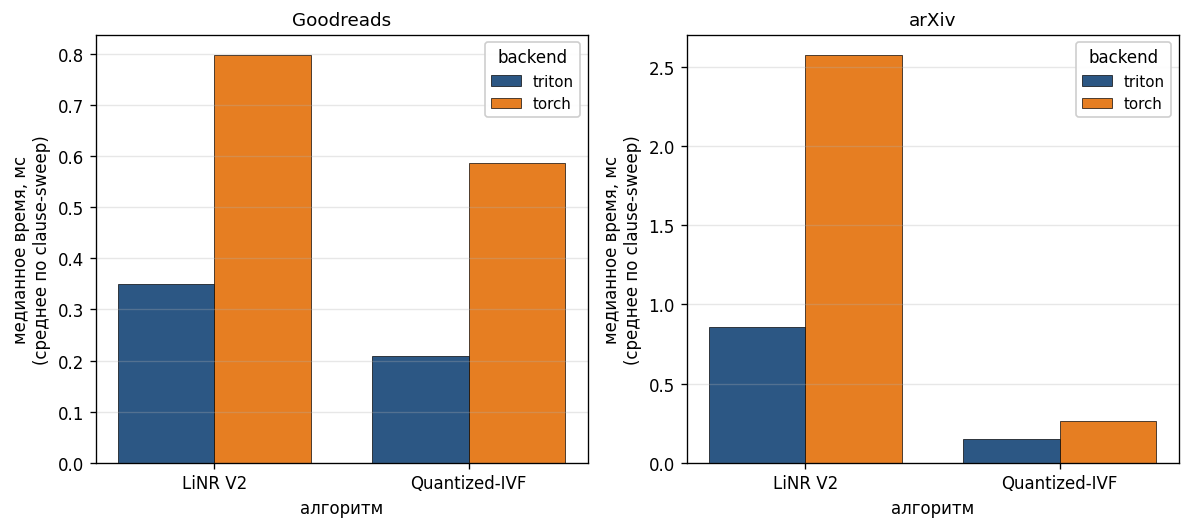
\includegraphics[width=0.9\textwidth]{figures/fig-4-1-backend-speedup.png}
    \caption{Медианное ускорение реализации на Triton относительно реализации на PyTorch.}
    \label{fig:backend_speedup}
\end{figure}

\textbf{Автоматический подбор параметров ядер.} В библиотеке реализован механизм автонастройки (autotuning) параметров вычислительных ядер, доступный в виде отдельной CLI-команды. Этот инструмент позволяет находить оптимальную конфигурацию размеров блоков (block sizes) и количества варпов (num\_warps) для конкретных условий эксплуатации: размера каталога, размера батча при инференсе и размерности эмбеддингов. Процесс подбора выполняется однократно на этапе предварительной настройки (offline), что полностью исключает накладные расходы на JIT-компиляцию во время работы сервиса.

\chapterconclusions

Архитектура фреймворка \textbf{torchretrieve} успешно решает задачу создания гибкой, высокопроизводительной и полностью совместимой с экосистемой PyTorch библиотеки для поиска кандидатов. Соблюдение заложенных инженерных принципов достигается за счёт введения единого интерфейса \textbf{FilterModule}, наличия эталонного PyTorch-бэкенда для верификации вычислений и механизма предварительной автонастройки ядер. Использование \textbf{torch.compile} в связке с пользовательскими операторами Triton позволяет оптимизировать весь инференс-этап целиком, что позволяет объединить энкодер запроса и поисковый индекс в один экспортируемый PyTorch-граф.

% =========================================================
% Chapter 5
% =========================================================
\chapter{Экспериментальные данные и протокол оценки}

\section{Наборы данных}

\begin{table}[htbp]
    \caption{Сводные характеристики наборов данных.}
    \label{tab:datasets}
    \centering
    \begin{tabular}{lrrl}
        \toprule
        Набор & Объектов & Тестовых запросов & Источник эмбеддингов \\
        \midrule
        Goodreads        & $797\,043$ & $313\,178$ & gSASRec \\
        arXiv            & $2{,}99$ млн & $10\,000$  & Nomic-Embed-v1.5 \\
        Yambda-500M      & $3{,}06$ млн & $45\,932$  & gSASRec \\
        Yambda-5B        & $5{,}37$ млн & $459\,067$ & gSASRec \\
        \bottomrule
    \end{tabular}
\end{table}

\textbf{Goodreads} \cite{wan2018item, wan2019fine} --- публичный набор данных социальной сети для читателей. Наличие атрибутов различной гранулярности делает его отличным полигоном для тестирования алгоритмов со встроенной фильтрацией. В качестве атрибутов объектов выступают:
\begin{itemize}
  \item \textbf{C0 --- жанр} (10 категорий, например, \textit{fiction}, \textit{poetry});
  \item \textbf{C1 --- язык издания} (top-30 ISO-кодов);
  \item \textbf{C2 --- формат издания} (например, \textit{paperback}, \textit{audio});
  \item \textbf{C3 --- интервал года публикации}.
\end{itemize}
Комбинации этих атрибутов позволяют создавать условия фильтрации от слабых до крайне селективных.

\textbf{arXiv} \cite{clement2019arxiv} --- публичный набор данных научных работ. Для получения векторных представлений текстов статей применялся энкодер Nomic-Embed-v1.5 \cite{nussbaum2024nomic}. Как и Goodreads, этот набор обладает богатым набором атрибутов:
\begin{itemize}
  \item \textbf{C0 --- основная тематическая категория} (например, \textit{cs}, \textit{math});
  \item \textbf{C1 --- тип лицензии} (например, \textit{cc-by}, \textit{public-domain});
  \item \textbf{C2 --- интервал года публикации};
  \item \textbf{C3 --- количество версий статьи}.
\end{itemize}

\textbf{Yambda} \cite{yandex2025yambda} --- публичный набор данных музыкальных событий Yandex Music, используется в двух масштабах: 500M ($3{,}06$ миллиона треков) и 5B ($5{,}37$ миллиона треков). Данный набор применяется исключительно для оценки алгоритмов в режиме без фильтрации.

\section{Энкодеры и схемы разделения данных}

Для рекомендательных наборов данных (Goodreads, Yambda) применяется метод разделения на обучающую и тестовую выборки Global Temporal Split, делающий глобальную отсечку по времени во избежание проникновения информации из будущего в обучение модели. В случае Goodreads оценка проводится на $313\,178$ тестовых пользователях. Для набора Yambda тестовая выборка составляет $45\,932$ пользователя на масштабе 500M и $459\,067$ пользователей на масштабе 5B. 

На наборе arXiv формируется $10\,000$ тестовых запросов путем выделения по одной статье на каждый запрос. Этот сценарий имитирует задачу поиска похожих статей по их семантическому содержанию, которая часто возникает при анализе научной литературы.

\section{Фильтрация по атрибутам и порядок оценки качества}
Каждое условие фильтрации представляет собой логическое выражение --- равенство (или неравенство) атрибута объекта и атрибута запроса. 
Для набора данных Goodreads используются следующие сущности:
\begin{itemize}
\item \textbf{C0} --- жанр;
\item \textbf{C1} --- язык;
\item \textbf{C2} --- формат издания;
\item \textbf{C3} --- год публикации.
\end{itemize}
Также при оценке качества используется условие неравенства языку запроса и объединения условий:
\begin{itemize}
\item \textbf{C4} --- одновременная фильтрация по жанру и языку;
\item \textbf{C5} --- все четыре условия сразу.
\end{itemize}
Для набора данных arXiv используются следующие сущности:
\begin{itemize}
\item \textbf{C0} --- основная тематическая категория;
\item \textbf{C1} --- лицензия научной работы;
\item \textbf{C2} --- год публикации;
\item \textbf{C3} --- количество версий статьи.
\end{itemize}
Аналогично Goodreads, при оценке качества используются и объединения условий:
\begin{itemize}
\item \textbf{C4} --- одновременная фильтрация по категории и году публикации;
\item \textbf{C5} --- объединение всех условий.
\end{itemize}

Выбор этих условий мотивирован их селективностью (долей объектов, проходящих фильтр) --- например, условие \textbf{C0} на arXiv оставляет в рассмотрении $\approx 5$--$30\%$ каталога объектов, тогда как объединение условий \textbf{C5} обладает очень высокой селективностью и сужает поиск до $\lesssim 5\%$ каталога. Это позволяет наглядно увидеть проблему нехватки кандидатов при постфильтрации и сравнить алгоритмы по их точности в различных сценариях применения. 

В ходе исследования замеры метрик были произведены по всем конфигурациям параметров:
\begin{itemize}
\item \textbf{Набор данных:} Goodreads, arXiv, Yambda-500M, Yambda-5B.
\item \textbf{Размерность эмбеддингов:} $d \in \{64, 128, 256\}$.
\item \textbf{Алгоритм:} LiNR V1, V2, V3, V4 и QuantizedIVF.
\item \textbf{Методология фильтрации:} без фильтрации, точная фильтрация и приближенная (Блум-фильтры).
\item \textbf{Количество возвращаемых кандидатов:} $K \in \{100, 200, 400, 500, 1000\}$.
\item \textbf{Размер батча:} $B \in \{1, 8, 16\}$.
\item \textbf{Реализация алгоритма:} PyTorch или Triton.
\end{itemize}

\section{Метрики}

Метрики вычисляются для каждого запроса, после чего усредняются по всей тестовой выборке. Изначально в рамках исследования также использовалась метрика $\mathrm{NDCG@}K$, но поскольку её тренды полностью повторяли $\mathrm{Recall@}K$, в работе приводится только полнота ($\mathrm{Recall}$). Определение метрики стандартно для задачи информационного поиска \cite{thakur2021beir}:
\begin{equation}
\mathrm{Recall@}K(q) = \frac{|R_q \cap G_q|}{\min(K, |G_q|)},
\end{equation}
где:
\begin{itemize}
    \item $q$ --- эмбеддинг запроса;
    \item $K$ --- количество возвращаемых кандидатов;
    \item $R_q$ --- множество $K$ найденных объектов для запроса $q$;
    \item $G_q$ --- множество релевантных объектов для запроса $q$.
\end{itemize}

В экспериментах используются две различные методологии оценки:
\begin{itemize}
\item В \textbf{режиме со встроенной фильтрацией} измеряется алгоритмическая точность самого метода поиска. Эталоном (ground truth) здесь выступает набор из $K$ лучших объектов, полученный с помощью точного поиска KNN с применением того же фильтра. Этот режим используется на наборах Goodreads и arXiv.
\item В \textbf{режиме без фильтрации} оценивается итоговое качество рекомендаций. Эталоном служат реальные отложенные взаимодействия пользователей с объектами. Этот режим применяется на наборах Goodreads и Yambda, чтобы показать, как итоговая полнота зависит от выбранного алгоритма и размерности эмбеддингов.
\end{itemize}

\section{Методология замеров скорости и памяти}

\begin{itemize}
    \item \textbf{Стенд.} Замеры выполнены на изолированном сервере с одной видеокартой NVIDIA A100-SXM4-80GB ($80$ ГБ памяти HBM2e, пропускная способность $2{,}04$ ТБ/с). На время замеров на сервере не выполняются никакие сторонние задачи.
    \item \textbf{Изоляция и прогрев.} Каждая конфигурация (датасет, размерность, размер батча, фильтр, реализация) запускается в отдельном Python-процессе, что изолирует кэш компиляции \textbf{torch.compile}, компиляцию Triton и аллокатор видеопамяти между алгоритмами. Перед каждым измерением выполняется $W = 20$ итераций прогрева алгоритма для JIT-компиляции ядер и стабилизации аллокатора.
    \item \textbf{Замер.} Тайминг выполняется через \texttt{triton.testing.do\_bench} на наборе из $4\,096$ батчей запросов. В работе представлено медианное время исполнения $t_\mathrm{med}$. Ускорение метода $A$ относительно метода $B$ определяется как $\mathrm{Speedup}(A,B) = t_\mathrm{med}(B) / t_\mathrm{med}(A)$.
    \item \textbf{Память.} Размер индекса вычисляется как общий размер всех тензоров модуля поиска и фильтрации. Пиковое потребление видеопамяти замеряется через \texttt{torch.cuda.max\_memory\_allocated()} в отдельном окне в $16$ повторов и включает временные буферы алгоритма.
    \item \textbf{Конфигурация компиляции.} Используется \textbf{torch.compile(mode="reduce-overhead", dynamic=True)}.
\end{itemize}

\chapterconclusions

Разработанный протокол оценки опирается на три разнообразных набора данных, что позволяет всесторонне протестировать алгоритмы. Выбранные условия фильтрации охватывают весь рабочий диапазон селективности --- от широких до крайне узких фильтров. Это дает возможность детально оценить поведение методов под разной нагрузкой. Использование изолированных процессов и режима \textbf{reduce-overhead} при компиляции гарантирует минимальные затраты памяти и высокую скорость работы. Все конфигурации экспериментов и эталонные результаты выложены в открытый доступ, что делает результаты, представленные в следующей главе, полностью прозрачными и воспроизводимыми.

% =========================================================
% Chapter 6
% =========================================================
\chapter{Результаты экспериментов}

В исследовании используются два режима оценки. В режиме со встроенной фильтрацией измеряется алгоритмическая точность --- то есть насколько хорошо приближённый алгоритм воспроизводит ответ точного поиска. В режиме без фильтрации эталоном выступают реальные пользовательские взаимодействия, что позволяет оценить влияние алгоритма на итоговое качество рекомендаций.

\section{Зависимость полноты от алгоритма в режиме без фильтрации}

В таблице \ref{tab:recall_nofilter} приведены значения Recall@100 для эмбеддингов размерности $d = 128$ при размере батча $B = 1$ с использованием оптимизированной реализации на Triton.

\begin{table}[htbp]
    \caption{Recall@100 относительно пользовательских действий (без фильтрации)}
    \label{tab:recall_nofilter}
    \centering
    \begin{tabular}{lcccc}
        \toprule
        Набор данных & LiNR V1 & LiNR V4 & LiNR V3 & QuantizedIVF \\
        \midrule
        Goodreads & $0{,}1479$ & $0{,}1478$ & $0{,}1438$ & $0{,}1449$ \\
        Yambda-500M & $0{,}1486$ & $0{,}1485$ & $0{,}1426$ & $0{,}1468$ \\
        Yambda-5B & $0{,}1779$ & $0{,}1778$ & $0{,}1590$ & $0{,}1739$ \\
        \bottomrule
    \end{tabular}
\end{table}

Квантизованный метод LiNR V4 демонстрирует маленькую потерю полноты по сравнению с базовым точным поиском (LiNR V1). В целом, все приближенные методы сохраняют высокую алгоритмическую полноту в режиме без фильтрации: LiNR V3 и QuantizedIVF удерживают не менее $\approx 97\%$ качества базового метода. Единственным исключением стал LiNR V3 на наборе Yambda-5B, поскольку фиксированный пул в 5000 кандидатов составляет менее $0{,}1\%$ от каталога в 5,37 млн уникальных треков, чего не хватает для высокой полноты на этапе грубого 1-битного ранжирования.

\section{Парето-кривые качества, скорости и памяти в режиме с фильтрацией}

В таблицах \ref{tab:pareto_arxiv} и \ref{tab:pareto_goodreads} обобщены показатели качества, скорости и потребления памяти на наборах arXiv и Goodreads ($d=128$, $K=100$, $B=1$). Представлены два среза: по широкому условию \textbf{C0} (основная тематическая категория) и по строгому условию \textbf{C5} (объединение четырех фильтров). Небольшое отклонение полноты точного метода LiNR V1-V2 от идеальной единицы (менее $1\%$) объясняется погрешностью округления при вычислениях в формате FP16 по сравнению с эталонным результатом в FP32.

\begin{table}[htbp]
    \caption{Результаты качества, времени работы и памяти на arXiv ($d=128$, $K=100$, $B=1$).}
    \label{tab:pareto_arxiv}
    \centering
    \begin{tabular}{llcccc}
        \toprule
        Условие & Алгоритм & Полнота & $t_\mathrm{med}$ (мс) & Ускорение & Память (МиБ) \\
        \midrule
        \textbf{C0} & LiNR V1 & $0{,}9923$ & $1{,}42$ & $1{,}00\times$ & $730$ \\
        & LiNR V2 & $0{,}9885$ & $0{,}85$ & $1{,}68\times$ & $730$ \\
        & LiNR V4 & $0{,}9539$ & $2{,}03$ & $0{,}70\times$ & $365$ \\
        & LiNR V3 & $0{,}6756$ & $1{,}31$ & $1{,}08\times$ & $775$ \\
        & QuantizedIVF & $0{,}8828$ & $0{,}15$ & $\mathbf{9{,}40\times}$ & $419$ \\
        \midrule
        \textbf{C5} & LiNR V1 & $0{,}9940$ & $1{,}43$ & $1{,}00\times$ & $730$ \\
        & LiNR V2 & $0{,}9914$ & $0{,}81$ & $1{,}76\times$ & $730$ \\
        & LiNR V4 & $0{,}9654$ & $2{,}02$ & $0{,}71\times$ & $365$ \\
        & LiNR V3 & $0{,}9159$ & $1{,}30$ & $1{,}10\times$ & $775$ \\
        & QuantizedIVF & $0{,}7611$ & $0{,}15$ & $\mathbf{9{,}47\times}$ & $427$ \\
        \bottomrule
    \end{tabular}
\end{table}
\begin{table}[htbp]
    \caption{Результаты качества, времени работы и памяти на Goodreads ($d=128$, $K=100$, $B=1$).}
    \label{tab:pareto_goodreads}
    \centering
    \begin{tabular}{llcccc}
        \toprule
        Условие & Алгоритм & Полнота & $t_\mathrm{med}$ (мс) & Ускорение & Память (МиБ) \\
        \midrule
        \textbf{C0} & LiNR V1 & $0{,}9968$ & $0{,}462$ & $1{,}00\times$ & $195$ \\
        & LiNR V2 & $0{,}9941$ & $0{,}347$ & $1{,}33\times$ & $195$ \\
        & LiNR V4 & $0{,}9648$ & $0{,}625$ & $0{,}74\times$ & $97$ \\
        & LiNR V3 & $0{,}7521$ & $0{,}390$ & $1{,}18\times$ & $207$ \\
        & QuantizedIVF & $0{,}9128$ & $0{,}211$ & $\mathbf{2{,}19\times}$ & $298$ \\
        \midrule
        \textbf{C5} & LiNR V1 & $0{,}9974$ & $0{,}462$ & $1{,}00\times$ & $195$ \\
        & LiNR V2 & $0{,}9952$ & $0{,}330$ & $1{,}40\times$ & $195$ \\
        & LiNR V4 & $0{,}9712$ & $0{,}624$ & $0{,}74\times$ & $97$ \\
        & LiNR V3 & $0{,}9587$ & $0{,}391$ & $1{,}18\times$ & $207$ \\
        & QuantizedIVF & $0{,}6014$ & $0{,}212$ & $\mathbf{2{,}18\times}$ & $298$ \\
        \bottomrule
    \end{tabular}
\end{table}

Анализ результатов позволяет выделить три основные закономерности. Во-первых, алгоритм QuantizedIVF уверенно занимает Парето-оптимальный фронт, обеспечивая ускорение на порядок (до $10{,}9\times$ на самых крупных каталогах) по сравнению с точным базовым методом. Во-вторых, LiNR V2 является доминирующим выбором, когда требуется максимальная полнота. В-третьих, LiNR V4 позволяет вдвое сократить потребление памяти, сохраняя при этом полноту на уровне $\geq 95\%$, если допустимо замедление в скорости ответа.

\begin{figure}[htbp]
    \centering
    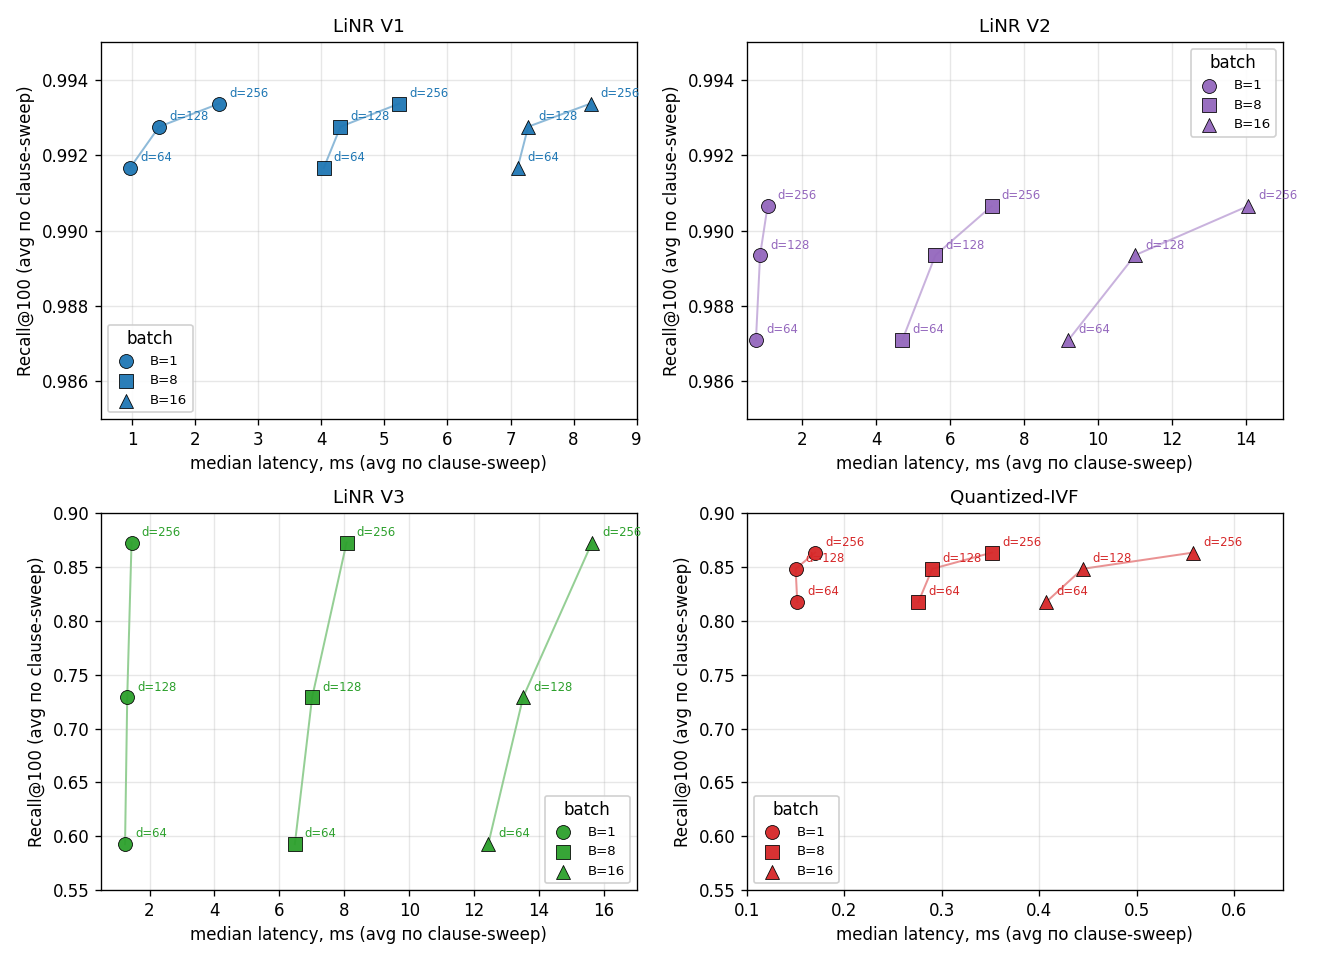
\includegraphics[width=0.9\textwidth]{figures/fig-6-1-pareto-quality-latency.png}
    \caption{Парето-кривые «полнота--скорость» на arXiv со встроенной фильтрацией ($d=128$, $K=100$, $B=1$).}
    \label{fig:pareto_quality_latency}
\end{figure}

\section{Влияние размера батча на скорость работы}

При обработке одиночных запросов ($B=1$) алгоритм LiNR V4 (INT8) уступает по скорости точным методам в формате FP16 (он медленнее V1 примерно в $1{,}4$ раза). Это связано с накладными расходами на построчный деквантизационный эпилог в INT32. Однако с увеличением размера батча эта разница быстро нивелируется: при $B=16$ время работы V4 практически сравнивается с V1 (отставание составляет всего $4\%$). Такое поведение объясняется более эффективной утилизацией тензорных ядер для целочисленного умножения и амортизацией накладных расходов при матричном умножении. Таким образом, LiNR V4 становится отличным выбором для высоконагруженных систем, обрабатывающих запросы батчами в условиях ограничений памяти.

В таблице \ref{tab:batch_scaling} приведены амортизированные задержки (медиана $t / B$, мс на один запрос) для набора arXiv при условии \textbf{C0}.

\begin{table}[htbp]
    \caption{Время работы (мс/запрос) при различных размерах батча $B$.}
    \label{tab:batch_scaling}
    \centering
    \begin{tabular}{lccc}
        \toprule
        Алгоритм & $B=1$ & $B=8$ & $B=16$ \\
        \midrule
        LiNR V1 & $1{,}42$ & $0{,}54$ & $\mathbf{0{,}45}$ \\
        LiNR V2 & $0{,}85$ & $0{,}69$ & $0{,}68$ \\
        LiNR V4 & $2{,}03$ & $0{,}58$ & $0{,}47$ \\
        LiNR V3 & $1{,}31$ & $0{,}88$ & $0{,}84$ \\
        QuantizedIVF & $\mathbf{0{,}15}$ & $\mathbf{0{,}04}$ & $\mathbf{0{,}03}$ \\
        \bottomrule
    \end{tabular}
\end{table}

Алгоритм QuantizedIVF сохраняет преимущество в скорости на порядок при любом размере батча. В то же время LiNR V2 и V3 довольно быстро достигают предела амортизации вычислений (см. рис. \ref{fig:batch_scaling}).

\begin{figure}[htbp]
    \centering
    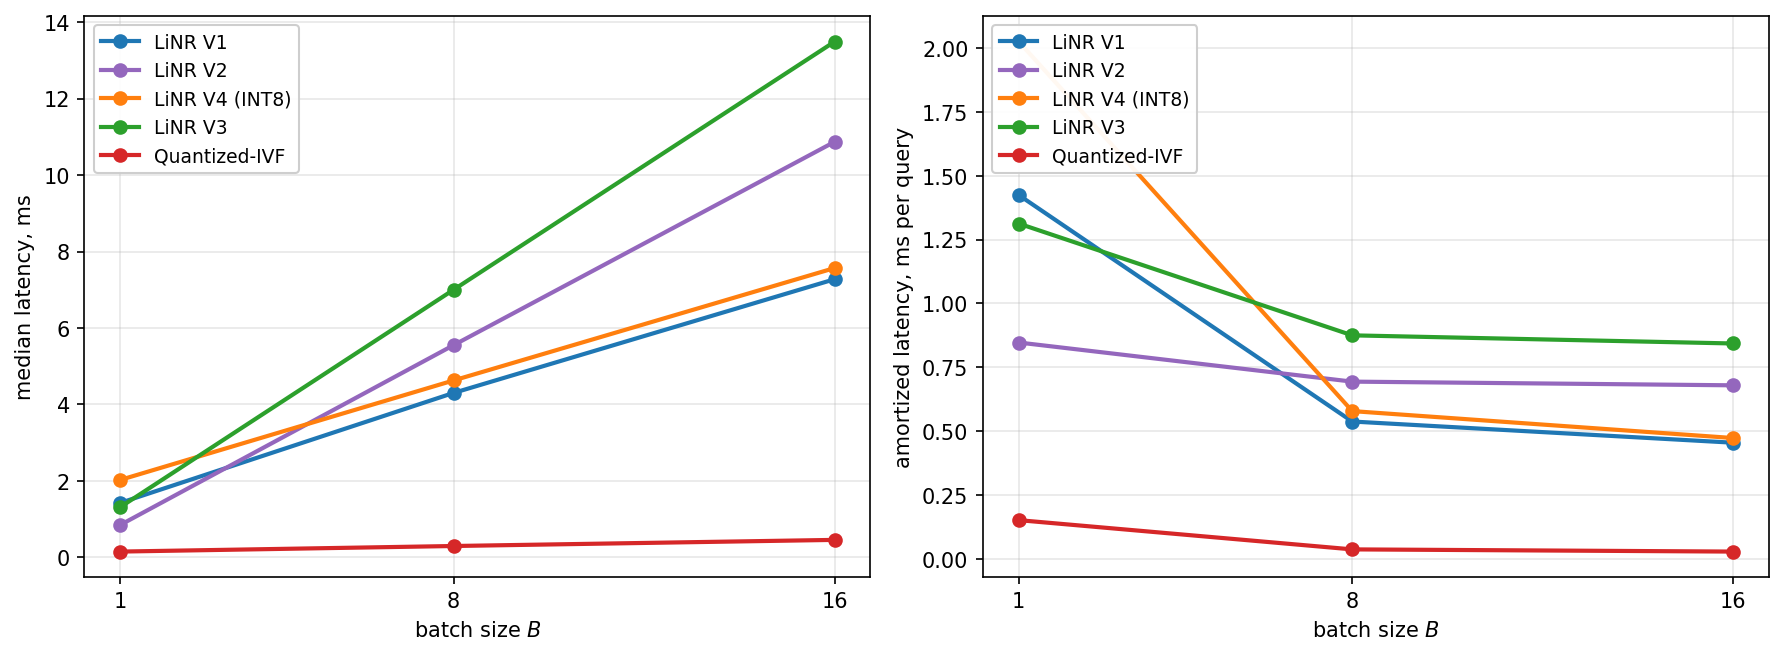
\includegraphics[width=0.9\textwidth]{figures/fig-6-3-batch-scaling.png}
    \caption{Зависимость амортизированной задержки от размера батча на arXiv (условие \textbf{C0}, $d=128$, $K=100$).}
    \label{fig:batch_scaling}
\end{figure}

\section{Масштабирование по размерности эмбеддинга}

Важным эксплуатационным аспектом является то, как время ответа меняется при увеличении размерности эмбеддингов $d$. На рис. \ref{fig:dim_scaling} представлены результаты измерений скорости поиска кандидатов для $d \in \{64, 128, 256\}$.

\begin{figure}[htbp]
    \centering
    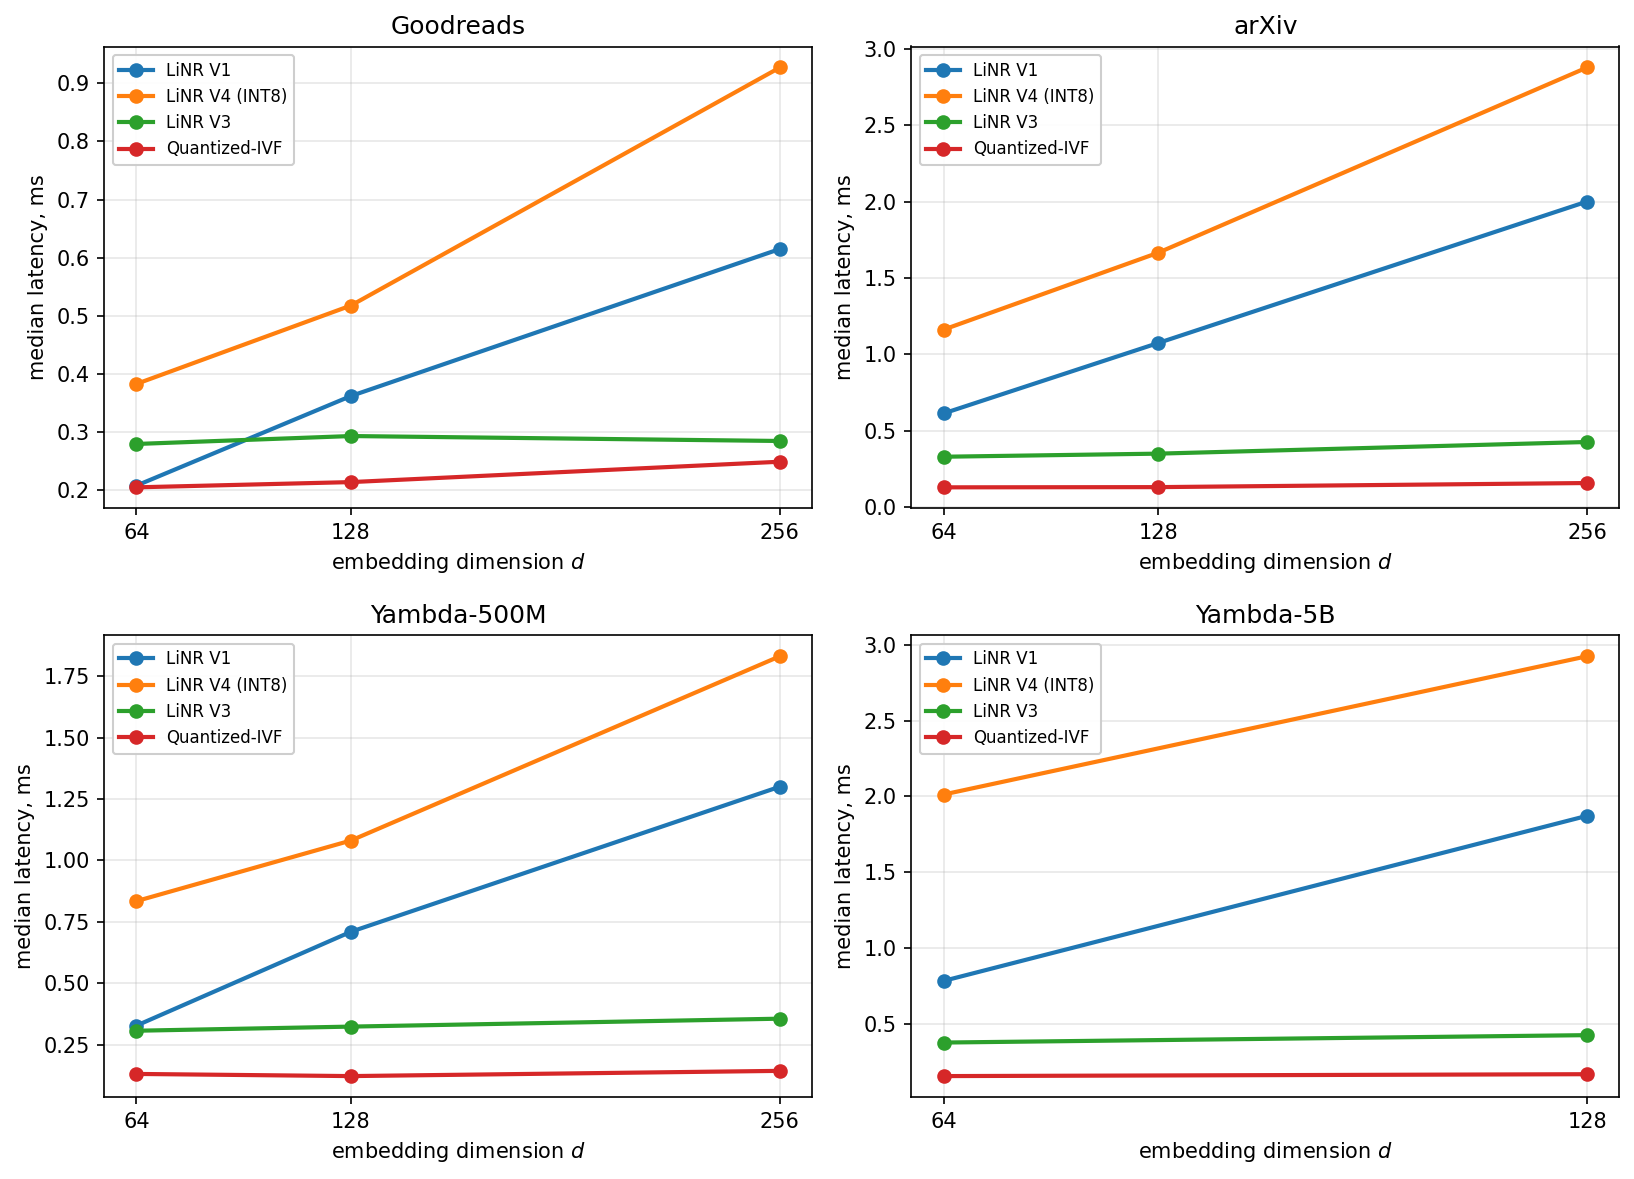
\includegraphics[width=0.95\textwidth]{figures/fig-6-9-dim-scaling.png}
    \caption{Зависимость скорости от размерности эмбеддинга $d$.}
    \label{fig:dim_scaling}
\end{figure}

Как видно из графиков, время работы точного алгоритма LiNR V1 растет практически линейно вместе с размерностью. Это происходит потому, что при одиночных запросах ($B=1$) его скорость жестко ограничена пропускной способностью видеопамяти (HBM) при считывании FP16-векторов. Квантизованный вариант LiNR V4 (INT8) также замедляется, но не так сильно, поскольку считывает в два раза меньше данных.
В то же время приближённые алгоритмы (LiNR V3 и QuantizedIVF) оказались почти нечувствительны к росту размерности. Почти плоский график QuantizedIVF объясняется тем, что фильтры Блума и IVF-кластеризация отсекают подавляющее большинство кандидатов еще до чтения самих векторов из памяти. На практике это означает, что при переходе от $d=64$ к $d=256$ точный поиск замедлится почти в 4 раза (или чуть меньше при лучшей утилизации GPU на больших батчах), тогда как время работы QuantizedIVF практически не изменится.

\section{Память индекса по алгоритмам}

Объем потребляемой памяти индекса зависит исключительно от размера каталога, размерности эмбеддингов и выбранного алгоритма. В таблице \ref{tab:memory} приведен сравнительный анализ для $d=128$.

\begin{table}[htbp]
    \caption{Размер индекса (МиБ) при $d=128$.}
    \label{tab:memory}
    \centering
    \begin{tabular}{lcccc}
        \toprule
        Датасет & LiNR V1 & LiNR V4 & LiNR V3 & QuantizedIVF \\
        \midrule
        Goodreads & $194{,}6$ & $97{,}3$ & $206{,}8$ & $297{,}8$ \\
        arXiv & $730{,}0$ & $364{,}9$ & $775{,}3$ & $418{,}7$ \\
        Yambda-500M & $456{,}0$ & $227{,}8$ & $484{,}1$ & $254{,}9$ \\
        Yambda-5B & $1310{,}0$ & $654{,}6$ & $1391{,}0$ & $800{,}3$ \\
        \bottomrule
    \end{tabular}
\end{table}

Как видно из таблицы, LiNR V4 занимает примерно в два раза меньше памяти по сравнению с LiNR V1. Алгоритм QuantizedIVF, который использует аналогичный метод квантизации, имеет дополнительные накладные расходы в виде хранения в памяти центроидов кластеров и 1024-битных Блум-фильтров для каждого объекта, благодаря которым он работает быстрее.  

\begin{figure}[htbp]
    \centering
    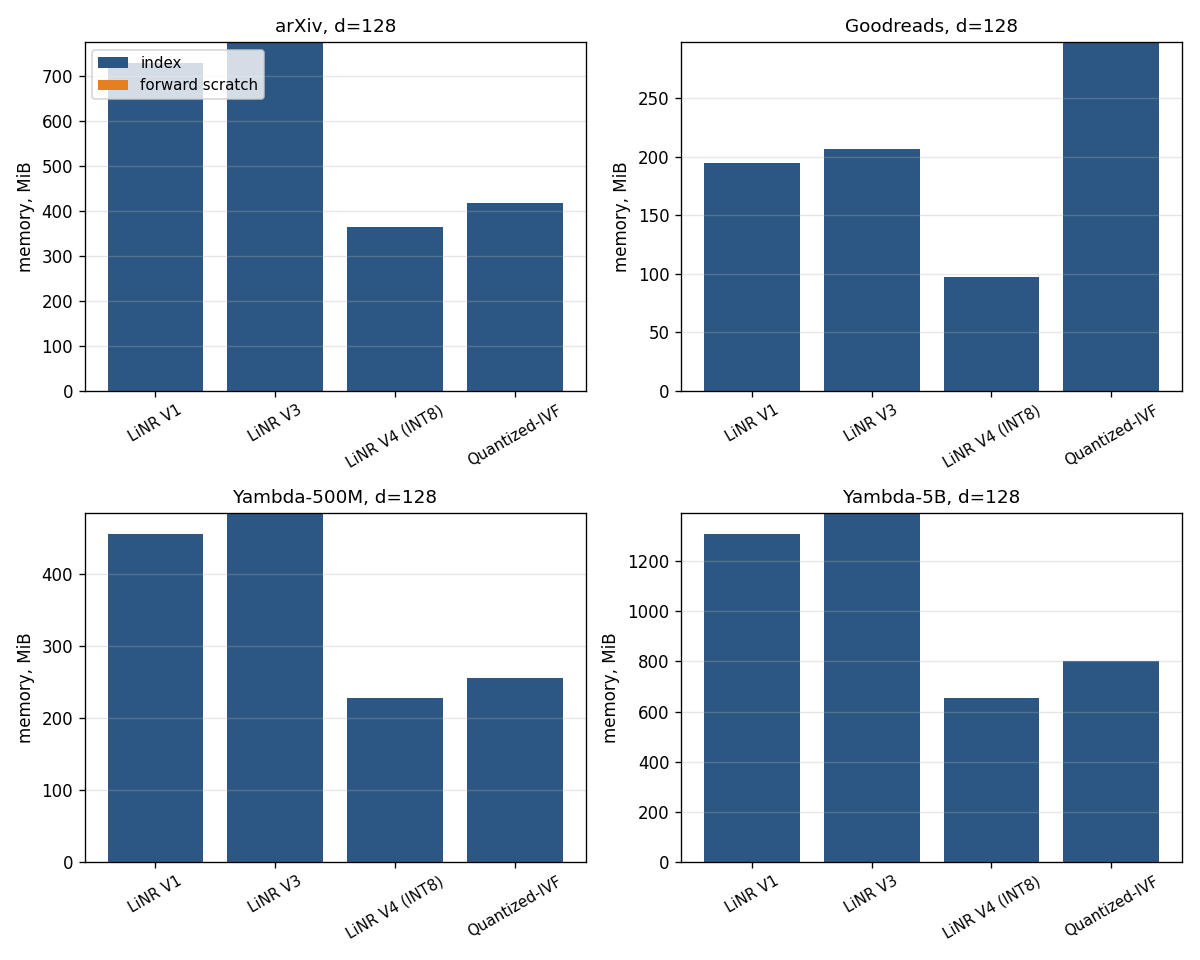
\includegraphics[width=0.9\textwidth]{figures/fig-6-4-memory-per-algo.png}
    \caption{Объем памяти индекса ($d=128$).}
    \label{fig:memory_per_algo}
\end{figure}

\section{Устойчивость алгоритмов к селективности фильтра}

На рис. \ref{fig:selectivity_recall} показана зависимость полноты от селективности фильтра, от самого слабого \textbf{C3} (пропускает $\approx 65\%$ каталога) до самого селективного \textbf{C5} (пропускает $\approx 4\%$), для различных алгоритмов при фиксированных параметрах.

\begin{figure}[htbp]
    \centering
    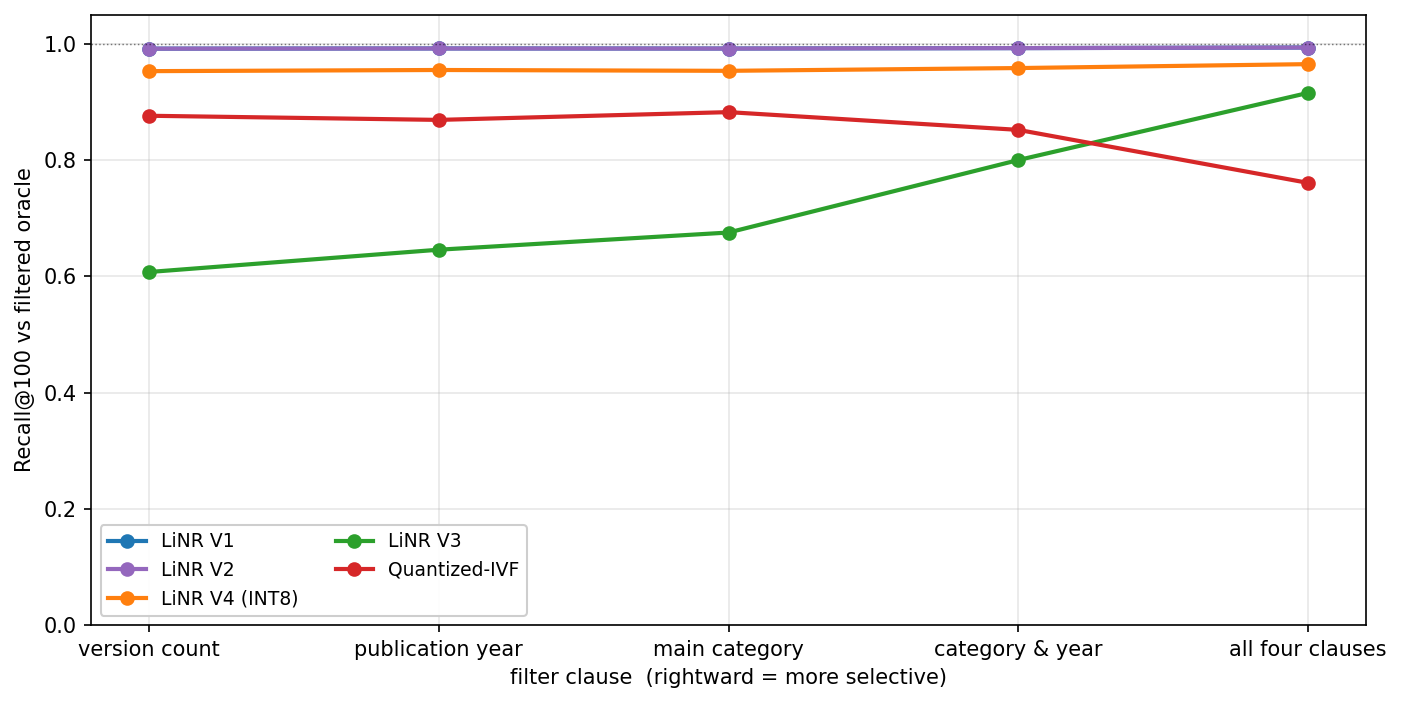
\includegraphics[width=0.9\textwidth]{figures/fig-6-5-selectivity-recall.png}
    \caption{Зависимость полноты от селективности условия arXiv ($d=128$, $K=100$, $B=1$).}
    \label{fig:selectivity_recall}
\end{figure}

Поведение алгоритмов можно разделить на три группы:

\textbf{Точные методы} (LiNR V1, V2 и квантизованный V4) демонстрируют стабильно высокую полноту, так как они вне зависимости от условия рассчитывают расстояния до всех объектов, прошедших фильтрацию. Различие между ними в таких сценариях заключается в скорости, так как при очень высокой селективности значительный объем вычислений, проводимый в алгоритме V1, делается впустую (или просто становится невозможен в виду размера каталога).

\textbf{QuantizedIVF} подвержен классической проблеме нехватки релевантных кандидатов (liquidity problem): при переходе от слабого фильтра к более сильному \textbf{C5} полнота падает с $0{,}88$ до $0{,}76$. Это связано с тем, что алгоритм просматривает не весь каталог, а лишь $n_\mathrm{probe}$ ближайших к эмбеддингу запроса кластеров. При строгом фильтре большинство объектов в этих кластерах не проходит фильтрацию и релевантных кандидатов не хватает для итогового списка; это можно компенсировать увеличением параметра $n_\mathrm{probe}$, разменивая скорость на полноту.

\textbf{LiNR V3} (Sign-OPORP с пулом $P_c=5000$) показывает обратное поведение: его полнота растет при ужесточении фильтра (с $0{,}67$ до $0{,}92$). В отличие от IVF, этот метод выполняет полный перебор каталога на этапе 1-битного ранжирования. Пула в 5000 кандидатов хватает, чтобы вместить почти все объекты, проходящие строгий фильтр \textbf{C5}. При широком же фильтре полнота ограничивается базовой точностью 1-битного хеша. Стоит отметить, что при существенном уменьшении пула $P_c$ алгоритм V3 также столкнется с нехваткой кандидатов.

\section{Замеры качества и скорости при различных параметрах алгоритмов}

Для выявления чувствительности двух аппроксимированных алгоритмов были проведены замеры точности, скорости и памяти алгоритмов в зависимости от их гиперпараметров.

\begin{figure}[htbp]
    \centering
    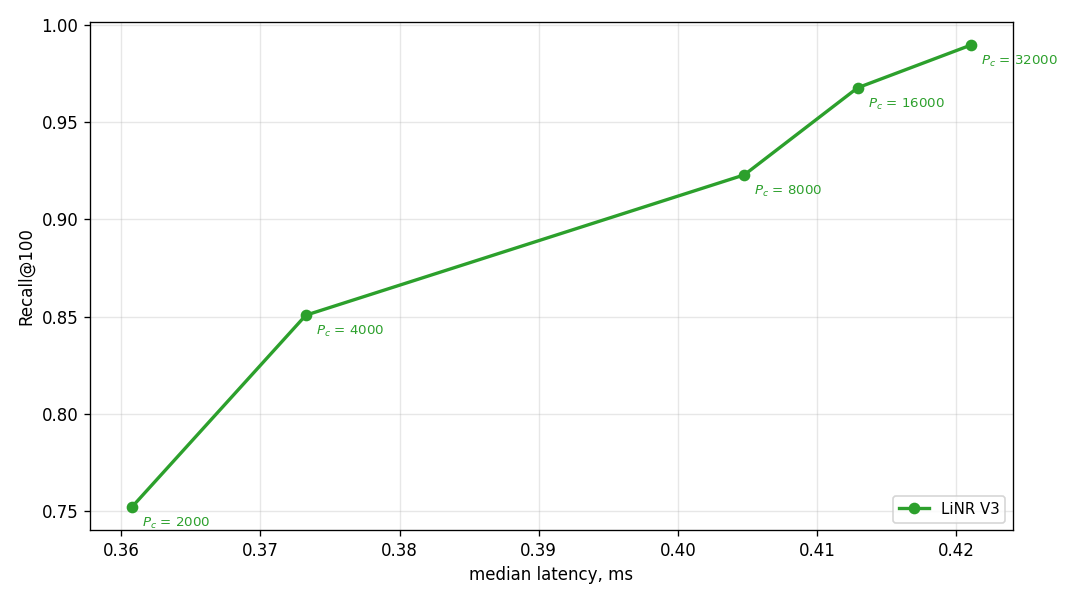
\includegraphics[width=0.9\textwidth]{figures/fig-6-6-linr-v3-pc-sweep.png}
    \caption{Зависимость полноты и времени работы LiNR V3 от размера пула кандидатов $P_c$ на Goodreads (условие \textbf{C0}, $d=128$, $K=100$).}
    \label{fig:linr_v3_pc_sweep}
\end{figure}

На рис. \ref{fig:linr_v3_pc_sweep} показано влияние размера множества кандидатов для переранжирования для алгоритма LiNR V3. Увеличение пула с 2000 до 32000 объектов позволяет восстановить Recall@100 практически до уровня эталонного решения ($\approx 0{,}99$). При этом рост времени ответа оказывается минимальным, что наглядно доказывает высокую эффективность побитового расчета расстояний над сжатыми эмбеддингами.

\begin{figure}[htbp]
    \centering
    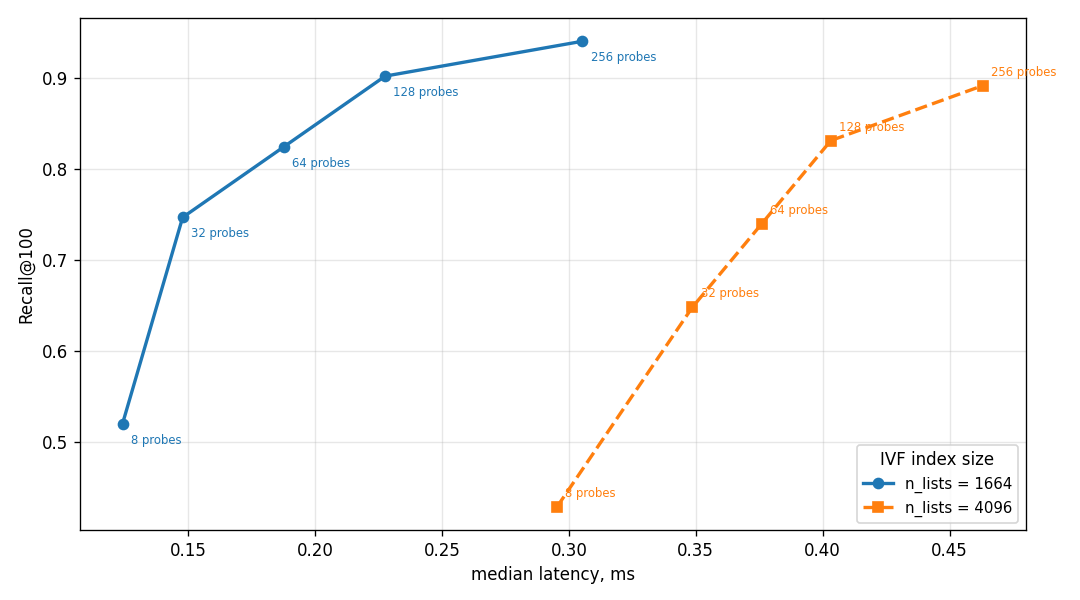
\includegraphics[width=0.9\textwidth]{figures/fig-6-7-silvertorch-pareto.png}
    \caption{Парето-кривые «полнота--скорость» алгоритма QuantizedIVF на arXiv (условие \textbf{C5}, $d=128$, $K=100$).}
    \label{fig:silvertorch_pareto}
\end{figure}

На рис. \ref{fig:silvertorch_pareto} представлены Парето-кривые для алгоритма QuantizedIVF при варьировании числа просматриваемых кластеров $n_\mathrm{probe}$ для двух разных разбиений каталога. Как видно из графика, конфигурация с мелкими кластерами ($n_\mathrm{lists} = 4096$) строго проигрывает конфигурации, близкой к классической эвристике $\sqrt{N}$ ($n_\mathrm{lists} = 1664$), как по полноте, так и по времени работы. 

Такое поведение объясняется аппаратными особенностями GPU: при избыточном дроблении каталога в каждом кластере оказывается слишком мало векторов. В результате накладные расходы на поиск ближайших центроидов, сортировку и запуск ядер для множества мелких блоков памяти перевешивают экономию от сокращения объема сканируемых данных. Таким образом, разбиение $n_\mathrm{lists} \approx \sqrt{N}$ формирует оптимальный Парето-фронт, обеспечивая наилучший баланс утилизации аппаратных ресурсов и качества поиска.

\chapterconclusions

Проведенное исследование позволяет сделать несколько выводов об эффективности алгоритмов поиска в разных сценариях. 

Во-первых, алгоритм \textbf{QuantizedIVF} продемонстрировал ускорение на порядок по сравнению с точным базовым методом при сохранении высокой полноты и с применением фильтрации, и без неё. Маленький размер индекса, высокая скорость и конфигурируемость делают этот метод оптимальным выбором по умолчанию для задач поиска по каталогам в миллионы объектов и выше.

Во-вторых, эксперименты подтвердили, что для сценариев с высокой селективностью фильтров лучше подходит алгоритм \textbf{LiNR V2} --- в таком случае расходы на материализацию промежуточной матрицы кандидатов минимальны и компенсируются экономией времени на расчете расстояний, при этом просматриваются все релевантные объекты из каталога, что позволяет решить проблему нехватки кандидатов при постфильтрации (liquidity problem).

В-третьих, алгоритм \textbf{LiNR V4} снижает размер индекса в два раза, позволяя уместить каталоги большего размера, и сохраняет высокую полноту ответа. При использовании батчинга запросов накладные расходы на квантизацию эмбеддинга запроса амортизируются за счет утилизации тензорных ядер, благодаря чему различия в скорости с точным поиском становятся минимальны.

% =========================================================
% Conclusion
% =========================================================
\chapter*{Заключение}
\addcontentsline{toc}{chapter}{Заключение}

В рамках работы исследованы и предложены методы быстрого поиска кандидатов на графических ускорителях для рекомендательных систем. Проведенный анализ показал, что существующие ANN-библиотеки плохо интегрируются в вычислительные графы современных нейросетей и зачастую не поддерживают эффективную атрибутную фильтрацию. Для решения этой проблемы был разработан открытый фреймворк \textbf{torchretrieve} на базе PyTorch и Triton.

В библиотеке воспроизведены промышленные алгоритмы семейства LiNR, а также предложены новые подходы: INT8-модификация LiNR V4 и новый алгоритм QuantizedIVF. Эксперименты на наборах данных Goodreads, arXiv и Yambda показали, что предложенные методы позволяют существенно сократить потребление видеопамяти и ускорить инференс на порядок. При этом алгоритмы с встроенной фильтрацией успешно решают проблему нехватки релевантных кандидатов, сохраняя высокую полноту поиска даже при очень жестких условиях фильтрации.

Таким образом, разработанный фреймворк предоставляет новые возможности для повышения скорости и эффективности рекомендательных систем. Использование языка Triton и бесшовная интеграция с \textbf{torch.compile} открывают перспективы для дальнейших исследований, включая разработку методов шардирования больших каталогов (multi-GPU) и потокового обновления индекса в реальном времени.

% =========================================================
% Bibliography
% =========================================================
\printbibliography[title={Библиографический список}]

\end{document}
